\documentclass[10pt]{article}
\usepackage[margin=0.8in]{geometry}
\usepackage[T1]{fontenc}\usepackage{lmodern,amsmath,booktabs,graphicx}
\usepackage[hidelinks]{hyperref}
\setlength{\parskip}{5pt}\setlength{\parindent}{0pt}
\title{SilentMethyl: supplementary analyses for the revised manuscript}
\author{}\date{}
\renewcommand{\thefigure}{S\arabic{figure}}
\begin{document}\maketitle
\textit{Working companion to main\_revised.tex. This file retains supporting results and separates superseded analyses from current-context evidence. Source-data packages and the bibliography were not attached and must accompany a submission.}

\section*{Supplementary Table S1. Methylation-level benchmarks}
Results on 26,570 held-out CpGs, recomputed on 19 September 2026 from \texttt{ablation\_breast\_epithelium/paired\_model\_bootstrap/model\_metrics\_recomputed.csv} and the retrained baseline metrics. Stochastic models are mean $\pm$ sample SD across seeds 42--44; ridge models have single values. These are not bootstrap confidence intervals. Every row uses the same SD convention; the earlier draft mixed sample and population SDs between rows, and its $M$ column for the context and fusion arms was carried over from the pre-swap MCF-10A run. CpGenie and DeepCpG were retrained on identical data, with DeepCpG restricted to its DNA module.
\begin{center}\small
\begin{tabular}{lrrr}\toprule
Model & $\beta$ MAE & $M$ MAE & ROC-AUC\\\midrule
Composition & 0.1954 & 1.9600 & 0.8748\\
$k$-mer ridge & 0.1565 & 1.6866 & 0.9190\\
Context & $0.1022\pm0.0000$ & $1.1763\pm0.0005$ & $0.9658\pm0.0000$\\
CpGenie & $0.1281\pm0.0013$ & $1.3858\pm0.0103$ & $0.9406\pm0.0006$\\
DeepCpG & $0.1253\pm0.0005$ & $1.3412\pm0.0112$ & $0.9437\pm0.0011$\\
Sequence & $0.1099\pm0.0008$ & $1.1941\pm0.0070$ & $0.9569\pm0.0007$\\
Fusion & $0.0914\pm0.0037$ & $1.0341\pm0.0289$ & $0.9744\pm0.0025$\\\bottomrule
\end{tabular}\end{center}
A displayed SD of 0.0000 reflects rounding, not deterministic training. All values were confirmed against the current prediction export. The old draft's claimed 20.8\% improvement over DeepCpG is inconsistent with these MAEs (the displayed values imply 27.1\%).

\section*{Supplementary Table S2. External evaluation units}
\begin{center}\small
\begin{tabular}{p{3.5cm}p{3.7cm}p{6.1cm}}\toprule
Analysis & Evaluation unit & Size / interpretation\\\midrule
GENOA signed test & Significant non-CpG-altering pair & 4,037 pairs; parent non-CpG-altering set 42,866\\
eGTEx signed test & Significant non-CpG-altering pair & 418 pairs; parent window-filtered set 76,893\\
eGTEx lead control & Lead variant--CpG association & 81 associations, 70 variants; selected stronger signals\\
eGTEx lead discrimination & Matched significant/high-$q$ pair & 35 matched pairs\\
Do--Tycko signed ASM & Index SNP, mean across scored DMR CpGs & 722 SNPs, 328 observed-positive, 179 blocks; seed 42\\
Rosenski ASM discrimination & Catalogue evaluation row & 6,910 rows, 242 blocks; bimodal non-ASM controls\\
Do--Tycko ASM discrimination & Catalogue evaluation row & 10,746 rows, 179 blocks; distance-matched non-DMR controls\\\bottomrule
\end{tabular}\end{center}
ASM discrimination AUROCs (fusion/sequence) were 0.5625/0.5736 in Rosenski and 0.5419/0.5432 in Do--Tycko. Distance-only baselines were 0.5017 (0.478--0.524) and 0.5030 (0.480--0.531), respectively. Catalogue-level rows are not independent participants. ASM intervals use 2,000 block resamples.

For Do--Tycko, sequence-only direction agreement was 0.5914 (0.554--0.629), signed Spearman 0.2503 (0.193--0.306), and directional AUROC 0.6308 (0.588--0.671). The mammary subset contained 53 SNPs; direction agreement was 0.5660 for both models with intervals spanning chance. A post-hoc restriction to 578 SNPs with observed effects of at least 20 percentage points increased direction agreement to 0.6055/0.6125. This restriction was not prospectively specified and does not erase the original 0.590 result's miss of the 0.60--0.70 expected band.

\section*{Supplementary Table S3. Context perturbation}
Agreement with the unperturbed seed-42 model on 76,893 pairs, from \texttt{ablation\_breast\_epithelium/context\_permutation/agreement\_with\_identity.csv}. The earlier draft reported this table from the pre-swap MCF-10A run. MAE/SD is deviation from the unperturbed prediction normalized by its standard deviation, not error against measured methylation. Sign agreement for levels and effects has different meanings.
\begin{center}\small
\begin{tabular}{llrrrr}\toprule
Scheme & Quantity & MAE/SD & Spearman & Sign & Pearson\\\midrule
Shuffle & Levels & 0.5260 & 0.6180 & 0.7522 & 0.6324\\
Shuffle & Effects & 0.2266 & 0.7755 & 0.8440 & 0.7528\\
Median & Levels & 0.3530 & 0.9430 & 0.9428 & 0.9525\\
Median & Effects & 0.1860 & 0.8047 & 0.8355 & 0.8624\\\bottomrule
\end{tabular}\end{center}
The original criterion used Pearson correlation and failed for median replacement. Normalized deviations and rank agreement characterize different aspects of sensitivity; they must not be substituted post hoc to claim that the original criterion passed.

\section*{Supplementary analysis 1. Error ranking and scale dependence}
Forward/reverse-complement disagreement was compared with three-seed variability, a boundary score $-|\widehat\beta-0.5|$, and a random control using error correlations and risk--coverage curves. The draft reports correlation with locus-level error near 0.50. Analyses were repeated on the $M$ scale and within predicted-$\beta$ strata (10, 20 and 50 strata in the reproduction record). The boundary score's apparent advantage weakened on the unbounded scale. This demonstrates scale dependence in error ranking; it neither supplies prediction intervals with verified coverage nor makes $M$-scale analysis the only valid assessment. Report both scales. Supplementary Fig.~\ref{fig:s1_uncertainty} shows these diagnostics from the current-context outputs.

\section*{Supplementary analysis 2. Motif and probe controls}
JASPAR CORE vertebrate motifs were scanned on both strands across 42,866 GENOA pairs. ALT scores were evaluated at the same offset and strand as the best REF occurrence. Per-factor correlations with $\Delta\widehat M$ were corrected for multiple testing; overlapping ETS matrices sharing the GGAA core should not be counted as independent mechanistic discoveries. The $k$-mer ridge reproduced these associations more strongly, while disruption magnitude was unrelated to predicted effect ($\rho=-0.011$). Composition, substitution and positional controls limit interpretation to motif/composition sensitivity. Supplementary Fig.~\ref{fig:s2_motifs} shows the neural and $k$-mer results together on a shared axis.

Only four test windows had nearest-training 31-mer Jaccard similarity above 0.5; excluding common-SNP-flagged probes left reported fusion MAE unchanged. These checks reduce specific concerns about overlap and probe artifacts but do not rule out all memorization or genotype confounding. Target coverage, mask exclusions and split counts should accompany their source data.

\section*{Supplementary analysis 3. Transfer and published-model comparisons}
The current-context lung transfer analysis reported distance-matched fusion AUROC 0.586 (0.565--0.607). This differs from the joint-training breast-held-out methylation-level test in the main paper.

The reproduction record identifies eight other tissue fusion scores and corresponding Melody comparisons as awaiting primary-epithelium rescoring. The earlier nine-tissue claim and eight-tissue fusion-versus-Melody comparisons are therefore not presented as current-model results. Sequence-only arms do not consume context and are unaffected by that swap, but a final comparison requires matched row sets, model versions and source exports.

The earlier Melody reanalysis suggested that benchmark identity explained more variation than prediction-track identity. It was exploratory. Nonsignificant differences in seven of eight tissues do not establish model equivalence; different windows, pretraining and tissue coverage prevent isolation of tissue matching alone. The shared-versus-tissue-specific mQTL analysis was sensitive to discovery power. That pattern is compatible with selection bias but does not prove winner's curse or locate all error in the benchmark. These analyses remain an optional supplementary extension after provenance reconciliation.

\section*{Supplementary analysis 4. Applications and clinical annotation}
NCOA2 remains a held-out synonymous hypothesis; STK11 remains an explicitly training-probe illustration. Current candidate scores are seed 42 only. Previously quoted three-seed candidate correlations, sign agreement and NCOA2 dispersion belong to the superseded context and are excluded.

For GWAS overlap, variants with a measured methylation association ($p<0.05$) were labeled by rsID or exact-coordinate overlap and matched on variant--CpG distance and allele frequency. Both cohorts were rescored against the current primary-breast-epithelium variant scores on 19 September 2026, giving 510 labeled eGTEx pairs and 573 GENOA pairs, unchanged from the earlier run because labelling depends on variant identity rather than on the model. The top-5\% GWAS fractions, 0.510 (0.271--0.679) in eGTEx and 0.561 (0.402--0.728) in GENOA, did not clearly exceed the matched null of 0.5. The published \texttt{gwas\_regulatory\_enrichment} run instead used every tested pair, including the roughly 71\% with no measured methylation effect, which script 52 documents as the wrong population for a regulatory claim; it is superseded by the two nominal runs reported here. GWAS annotation is an imperfect proxy for function, and this null result does not establish absence of disease-relevant methylation effects.

\section*{Supplementary figures}

Figures S1--S4 were generated by \texttt{scripts/95\_build\_revision\_figures.py} from the current
primary-breast-epithelium exports only. Each panel has a machine-readable source table under
\texttt{figures/source\_data/}, indexed with SHA-256 checksums in
\texttt{figures/source\_data/source\_data\_index.csv}. Colour is never the only encoding: marker shape
and line style repeat every model distinction, so the panels remain readable in grayscale.

\begin{figure}[htbp]
\centering
\IfFileExists{figures/figS1_uncertainty.pdf}{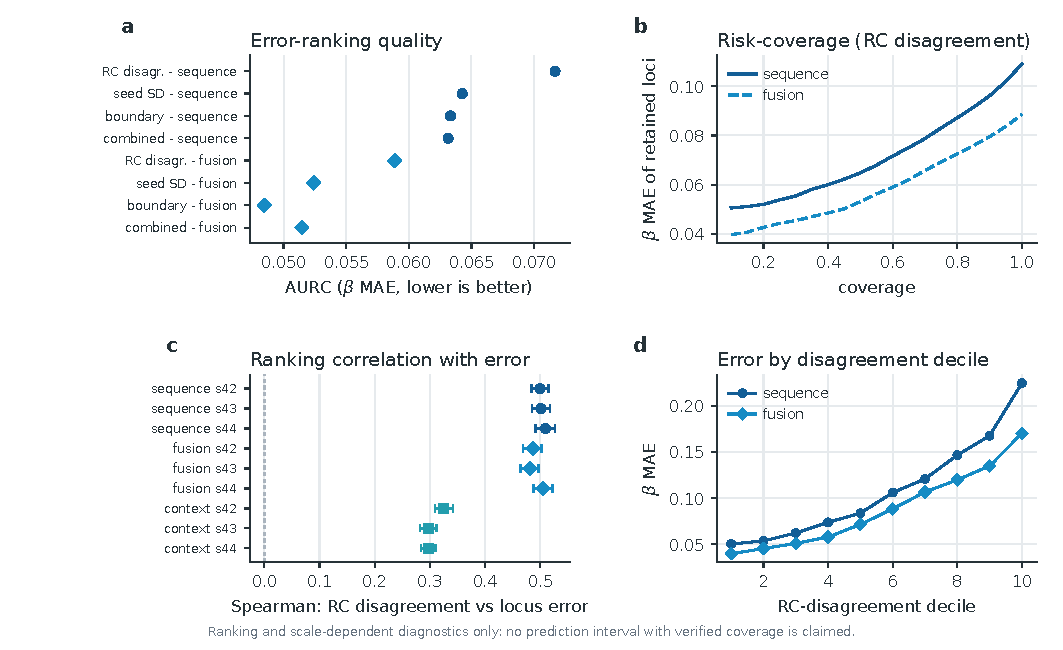
\includegraphics[width=\textwidth]{figures/figS1_uncertainty.pdf}}{\fbox{\parbox[c][40mm][c]{\textwidth}{\centering Supplementary Figure S1 not yet built}}}
\caption{\textbf{Error-ranking diagnostics.}
\textbf{a}, Area under the risk--coverage curve for four error-ranking scores at seed 42, for the
sequence and fusion models; lower is better and no interval is drawn because the summary export
carries none. \textbf{b}, Risk--coverage curves for reverse-complement disagreement on the same
retained loci and ranking direction. \textbf{c}, Spearman correlation between reverse-complement
disagreement and locus-level absolute error, for every model and seed; intervals are 1\,Mb genomic-block
bootstraps and the dashed line marks the null of zero. \textbf{d}, $\beta$ MAE by decile of
reverse-complement disagreement. All panels use $n=26{,}570$ held-out CpGs in 257 genomic blocks.
These are ranking and scale-dependent diagnostics: none of them supplies a prediction interval with
verified coverage.}
\label{fig:s1_uncertainty}
\end{figure}

\begin{figure}[htbp]
\centering
\IfFileExists{figures/figS2_motif_controls.pdf}{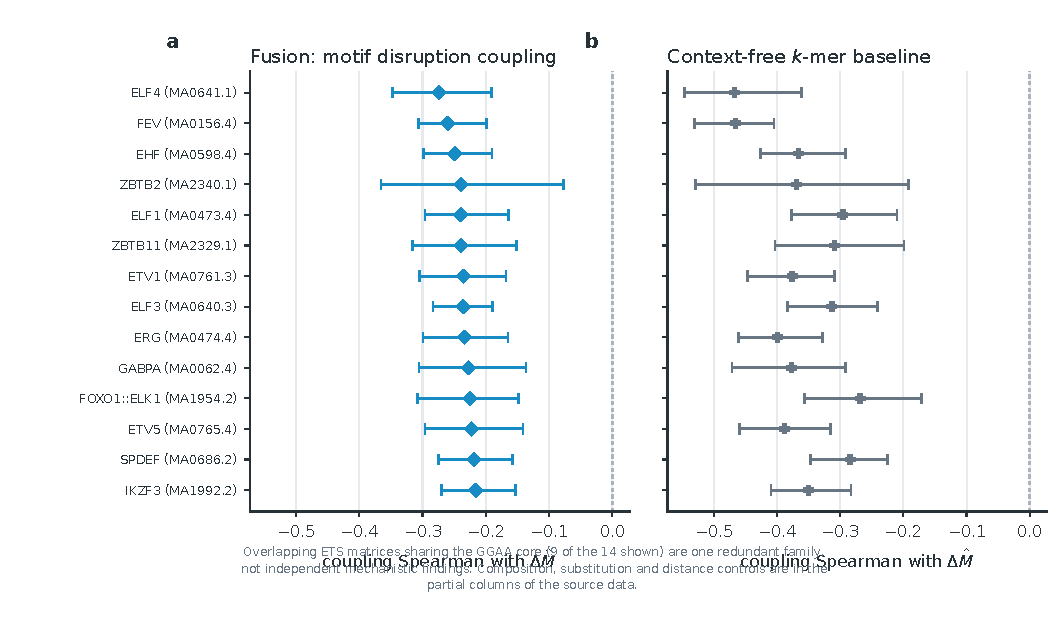
\includegraphics[width=\textwidth]{figures/figS2_motif_controls.pdf}}{\fbox{\parbox[c][40mm][c]{\textwidth}{\centering Supplementary Figure S2 not yet built}}}
\caption{\textbf{Motif-disruption controls.}
\textbf{a}, The 14 JASPAR CORE vertebrate matrices with the largest absolute coupling between motif
disruption and predicted $\Delta\widehat M$ under the fusion model. \textbf{b}, The same matrices scored
by the context-free $k$-mer ridge baseline on a shared axis. Points are Spearman correlations with
1\,Mb block-bootstrap intervals; the dashed line marks the null of zero, and per-matrix coverage counts
and block counts are in the source table. Overlapping ETS matrices share the GGAA core and are one
redundant family rather than independent mechanistic findings. Partial correlations controlling GC
content, variant--CpG distance and substitution class are reported as additional columns of the source
table rather than as separate panels.}
\label{fig:s2_motifs}
\end{figure}

\begin{figure}[htbp]
\centering
\IfFileExists{figures/figS3_target_split_qc.pdf}{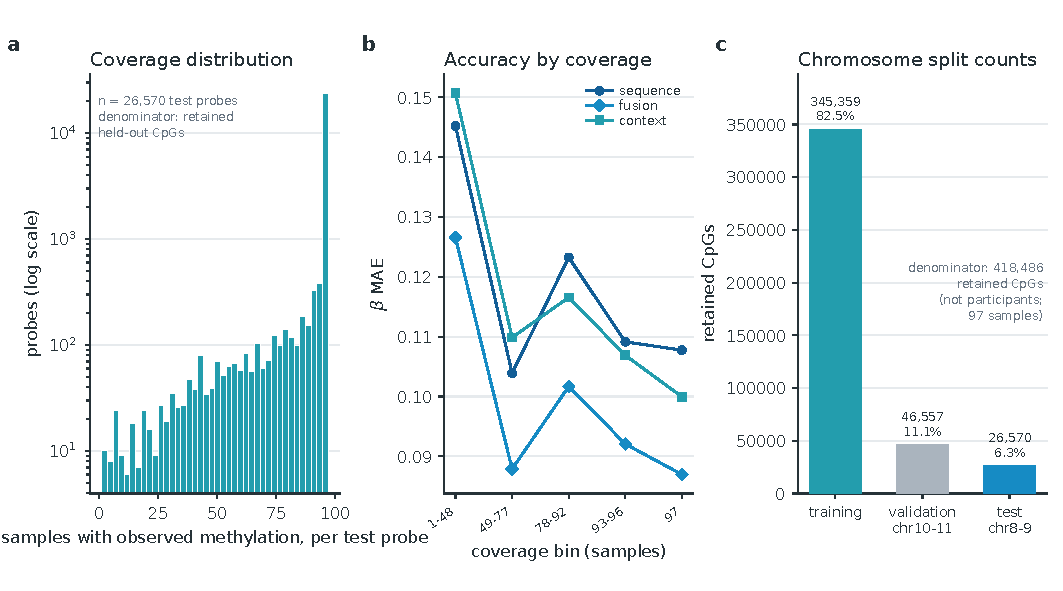
\includegraphics[width=\textwidth]{figures/figS3_target_split_qc.pdf}}{\fbox{\parbox[c][40mm][c]{\textwidth}{\centering Supplementary Figure S3 not yet built}}}
\caption{\textbf{Target construction and split QC.}
\textbf{a}, Number of samples contributing an observed methylation value to each held-out probe, on a
logarithmic count axis; the denominator is the 26,570 retained held-out CpGs. \textbf{b}, $\beta$ MAE by
coverage bin for the sequence, fusion and context models, so that accuracy can be read against target
support. \textbf{c}, Retained CpGs in each chromosome partition, with each percentage taken over the
418,486 retained CpGs. The split is by chromosome and not by participant: all 97 samples contribute to
every partition.}
\label{fig:s3_qc}
\end{figure}

\begin{figure}[htbp]
\centering
\IfFileExists{figures/figS4_external_controls.pdf}{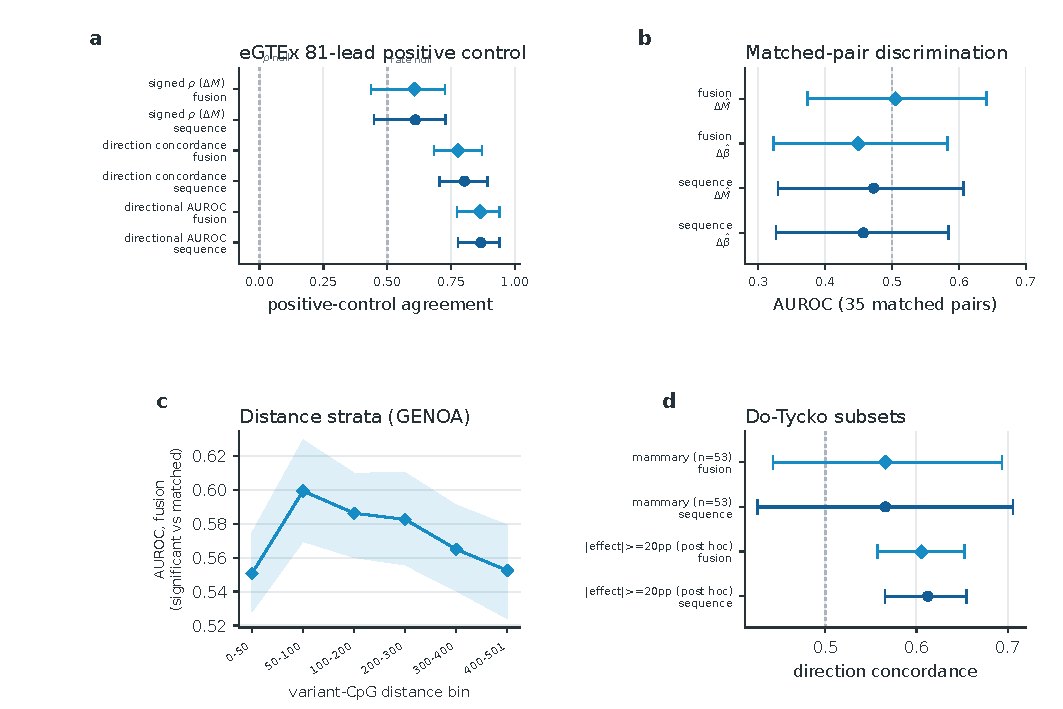
\includegraphics[width=\textwidth]{figures/figS4_external_controls.pdf}}{\fbox{\parbox[c][40mm][c]{\textwidth}{\centering Supplementary Figure S4 not yet built}}}
\caption{\textbf{Detailed external controls.}
\textbf{a}, The eGTEx lead-variant positive control on 81 associations from 70 variants: signed Spearman
correlation with the measured $\Delta M$, direction concordance and directional AUROC, for fusion and
sequence. Intervals are 10,000 bootstrap draws over variant-identifier clusters; the two dashed lines
give the correct null for each scale, zero for the correlation rows and 0.5 for the rate rows.
\textbf{b}, Discrimination between 35 matched significant and high-$q$ lead pairs, scored on predicted
$\Delta\widehat M$ and predicted $\Delta\widehat\beta$; intervals are 5,000 match-set bootstrap draws and
the null is 0.5. \textbf{c}, Fusion AUROC across GENOA variant--CpG distance strata, with block-bootstrap
bands. \textbf{d}, Do--Tycko direction concordance for the 53-SNP mammary subset and for the post-hoc
restriction to 578 SNPs with observed effects of at least 20 percentage points. The effect-size
restriction was not prespecified and is labelled as post hoc; it does not retract the
0.590 all-tissue result's miss of the recorded 0.60--0.70 band.}
\label{fig:s4_controls}
\end{figure}

\section*{Source-data and supplementary-figure assembly}
Figures~\ref{fig:s1_uncertainty}--\ref{fig:s4_controls} were built from the current primary-breast-epithelium exports by \texttt{scripts/95\_build\_revision\_figures.py}, which also writes one source-data table per panel with a SHA-256 index. Existing machine-readable packages S1--S12 retain their original identifiers; these are data-package sections, not the figure/table numbering used here. Merge and index the files at submission, preserve checksums and include the current candidate seed limitation. No new biological analysis was run in this editorial revision.
\end{document}
